\documentclass{article}
\usepackage{tempora}
\usepackage{indentfirst}
\usepackage{tabularx}
\usepackage{caption}
\usepackage{graphicx}
\usepackage{longtable}
\usepackage{tabularx}
\usepackage{amsmath}
\usepackage{amsfonts}
\usepackage{floatrow}
\floatsetup[table]{capposition=top}
\makeatletter
\graphicspath{ {./images/} }
\renewcommand*\l@section{\@dottedtocline{1}{1.5em}{2.3em}}
\makeatother
\usepackage{float}
\usepackage[english, russian]{babel}
\begin{document}
  \textbf{Постановка задачи}.

  Решается задача поиска оптимального распределения функционала программного средства по плагинам для интеграции в плагинную систему с уменьшенем связности его компонентов. При этом существуют ограничения на общее число используемых плагинов и на распределение функционала по ним. Функционал описан в требованиях к программному средству и реализован в файлах исходного кода на языке программирования.

  \begin{figure}[H]
      \centering
      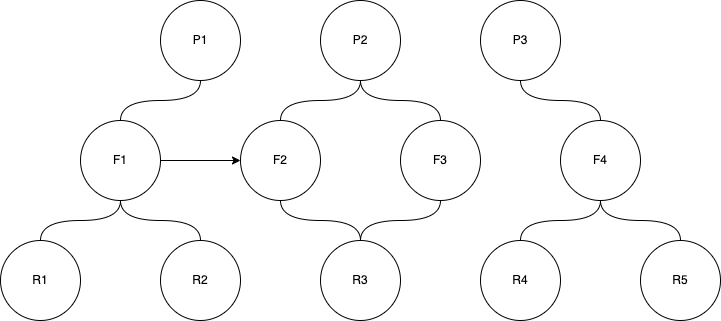
\includegraphics[width=1\textwidth]{Исходный граф.drawio}
      \caption{Граф $G$}
  \end{figure}

  Описание модели:
  \begin{itemize}
    \item Требования $R$ в количестве $n$ штук.
    \item Файлы исходного кода $F$ в количестве $m$ штук
    \item Плагины $P$ в количестве $k$ штук
    \item Требования трассируются на файлы исходного кода и образуется матрица связей $E_{rf} = m \times n$.
    \item Файлы исходного кода имеют друг на друга зависимости. Поэтому необходима матрица зависимостей $E_{ff} = m \times m$.
    \item Файлы исходного кода распределены по плагинам и образуется матрица связей $E_{fp} = k \times m$
  \end{itemize}

  Не все требования, реализованные в рамках поставки являются полезными для заказчика. Отношение числа бесполезных требований к общему числу требований, вошедшихх в поставку, называется коэффициентом бесполезности: $K_{un} = (\sum R' - \sum R_{n}) / \sum R'$, где:
  \begin{itemize}
    \item $R'$ - требования, реализованные в рамках поставки
    \item $R_{n}$ - полезные в рамках поставки требования
  \end{itemize}

  Для указания необходимых в поставке требований модель принимает на вход вектор $R$ элементов. Элементы на позициях соответствующих индексам полезных требований равны $1$, бесполезных - $0$.

  Например: $R_{n} = \{R_{1} = 1, R_{2} = 0, ..., R_{n} = 1\}$.

  Для определения $R'$ необходимо:
  \begin{enumerate}
    \item определить перечень полезных файлов исходного кода $F_n$. Чтобы требование было реализовано в рамках поставки необходимо включение всех файлов исходного кода на которые требование трассируется.

    $F_n = R_{n} \cdot E_{FR}$

    \item определить перечень файлов исходного кода с учетом разрешения зависимостей. Для этого нужно последовательно включать в поставку 

    \item если файл включен в поставку, соответствующий элемент вектора $F$ принимает значение $1$, иначе $0$. Для присвоения этими значениями вектор $F$ применяется функция активации: 

    $
    A_{F}(x) = 
      \begin{cases}
        0 & \quite \text{ если } x = 0
        1 & \quite \text{ если } x > 0
      \end{cases}
    $
  \end{enumerate}

  Необходимыми условиями трассируемости требований на файлы исходного кода является:
  \begin{itemize}
    \item каждое требование должно быть реализовано по меньшей мере в одном файле
    \item каждый файл реализует по меньшей мере одно требование
  \end{itemize}

  Признаком наличия связи требование-файл является ненулевое значение соответствующего элемента матрицы $E_{RF}$. Значение элемента равно $0$ если связь отсутствует. Чтобы выполнялись вышеописанные ограничения необходимо:
  \begin{itemize}
    \item сумма элементов в каждой строке матрицы была больше 0:
      \begin{itemize}
        \item $\sum^n_i E_{FR_{i, 1}} > 0$
        \item $\sum^n_i E_{FR_{i, 2}} > 0$
        ...
        \item $\sum^n_i E_{FR_{i, m}} > 0$
      \end{itemize}
    \item сумма элементов в каждом столбце матрицы была больше 0:
      \item $\sum^m_j E_{FR_{1, j}} > 0$
      \item $\sum^m_j E_{FR_{2, j}} > 0$
      \item ...
      \item $\sum^m_j E_{FR_{n, j}} > 0$
  \end{itemize}





  Задача сводится к поиску оптимального распределения файлов по плагинам. Для поиска оптимального распределения можно использовать выборки поставляемых требований. Всего существует $2^n - 1$ возможных выборок поставляемых требований. Возможные комбинации удобно записать в виде таблицы:
  \begin{table}[H]
    \caption{Table 1}
    \begin{center}
      \begin{tabular}[H]{|c|c|c|c|c|}
         n  & n - 1 & ... &  2  &  1  \\
         \hline
         0  &   0   & ... &  0  &  1  \\
         0  &   0   & ... &  1  &  0  \\
         0  &   0   & ... &  1  &  1  \\
        ... &  ...  & ... & ... & ... \\
         0  &   1   & ... &  0  &  0  \\
         0  &   1   & ... &  0  &  1  \\
         0  &   1   & ... &  1  &  0  \\
         0  &   1   & ... &  1  &  1  \\
        ... &  ...  & ... & ... & ... \\
         1  &   0   & ... &  0  &  0  \\
         1  &   0   & ... &  0  &  1  \\
         1  &   0   & ... &  1  &  0  \\
         1  &   0   & ... &  1  &  1  \\
        ... &  ...  & ... & ... & ... \\
         1  &   1   & ... &  0  &  0  \\
         1  &   1   & ... &  0  &  1  \\
         1  &   1   & ... &  1  &  0  \\
         1  &   1   & ... &  1  &  1  \\
      \end{tabular}
    \end{center}
  \end{table}

\end{document}
